\documentclass[10pt, compress]{beamer}

\usetheme[usetitleprogressbar,usetotalslideindicator]{m}

\usepackage{booktabs}
\usepackage[export]{adjustbox}
\usepackage[scale=2]{ccicons}

\usepgfplotslibrary{dateplot}

\title{Semantic micro-location maps}
\subtitle{for indoor localization of mobile app users}
\date{\today}
\author{Michal Rus}
\institute{Grzegorz J. Nalepa, PhD, DSc}

\begin{document}

\maketitle

\begin{frame}[fragile]
  \frametitle{Problem}
  \begin{block}{Micro-location}
  	Lokalizacja urządzenia wewnątrz budynku.
  \end{block}

  \begin{itemize}
  	\item GPS nie działa wewnątrz (osłabienie, 4+ sat., odbicia),
  	\item common-use devices nie mają dedykowanych rozwiązań,
  	\item efekty EM pogarszają znane \textasciitilde rozwiązania.
  \end{itemize}
\end{frame}

\begin{frame}[fragile]
	\frametitle{Rozwiązania}
	\begin{itemize}
		\only<1->{\item magnetyczne pozycjonowanie (dokł. 1÷2 metry z 90\% pewności)\only<2->{,}}
		\only<2->{\item pomiary inercjalne (krokomierz, \ldots)\only<3->{,}}
		\only<3->{\item bazujące na Wi-Fi\only<4->{,}}
		\only<4->{\item Bluetooth (iBeacons)\only<5->{,}}
		\only<5->{\item RFID, grid concepts, angle of arrival, time of arrival, ultrawide band, infrared, visible light communication, ultrasound, QR, NFC, \ldots}
	\end{itemize}
	\only<1>{\begin{figure}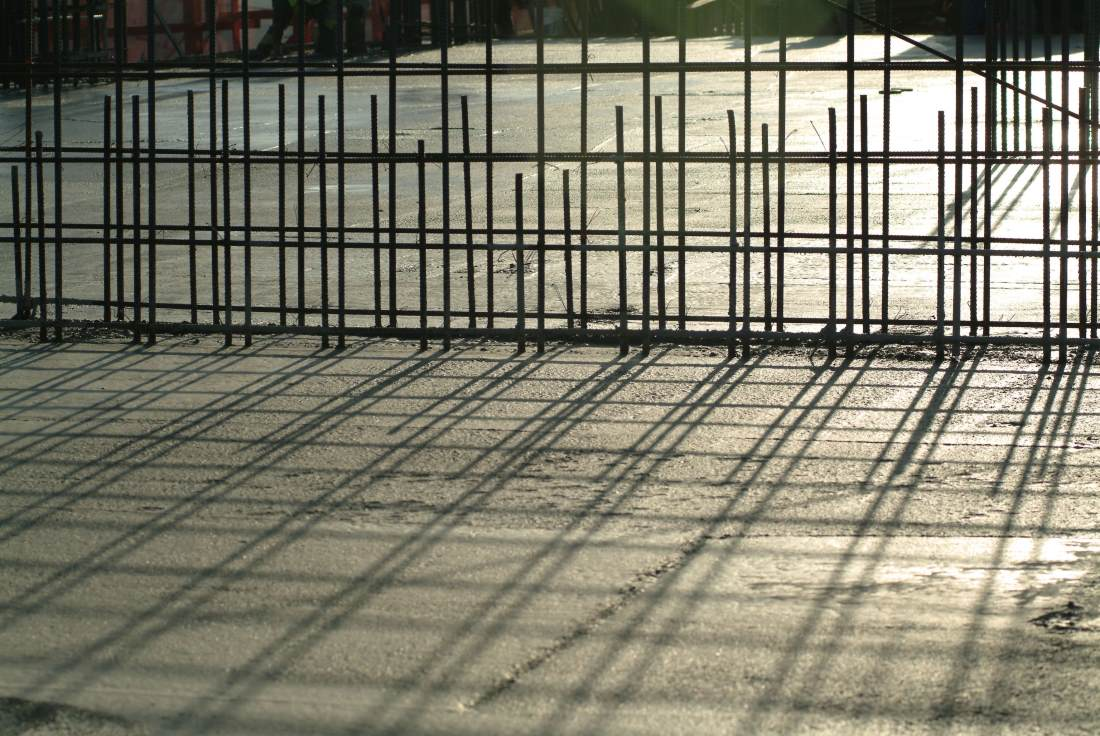
\includegraphics[width=.5\textwidth]{magnetic-positioning}\end{figure}}
	\only<2>{\begin{figure}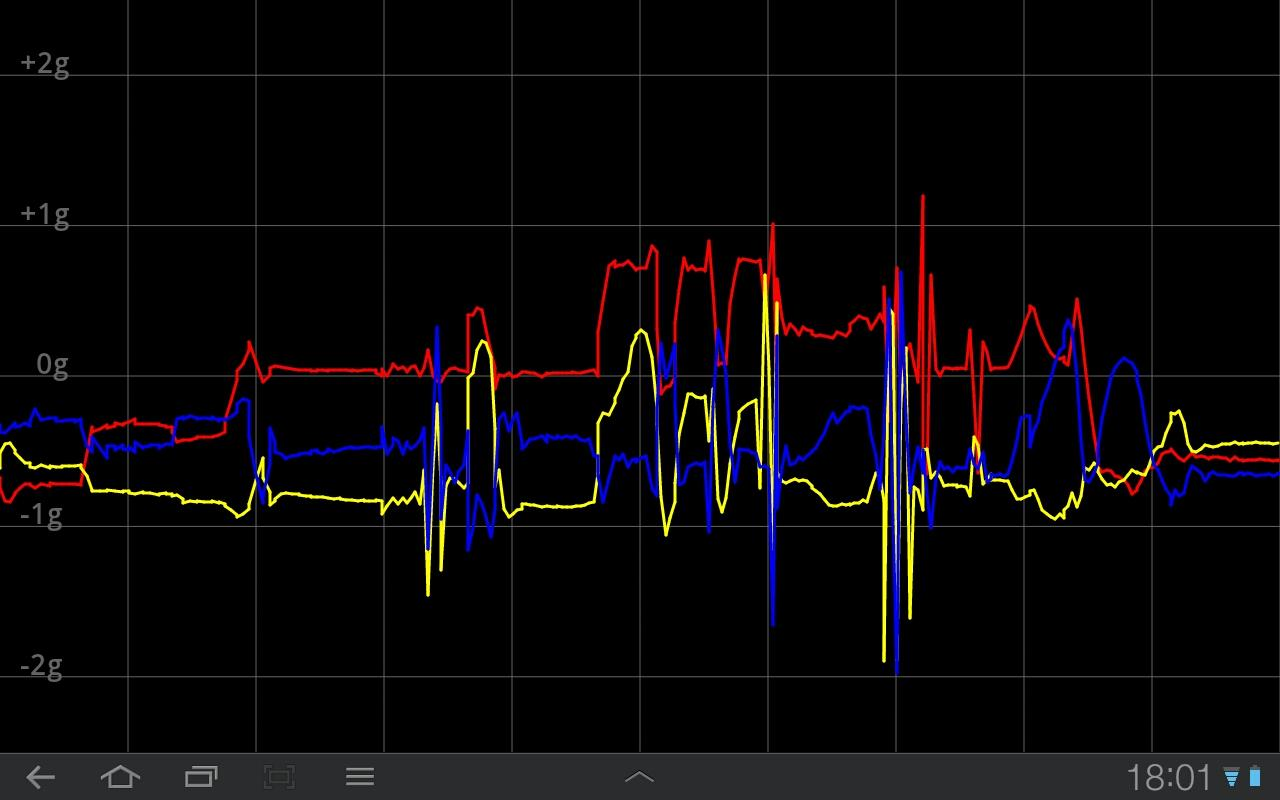
\includegraphics[width=.5\textwidth]{inertial-measurements}\end{figure}}
	\only<3>{\begin{figure}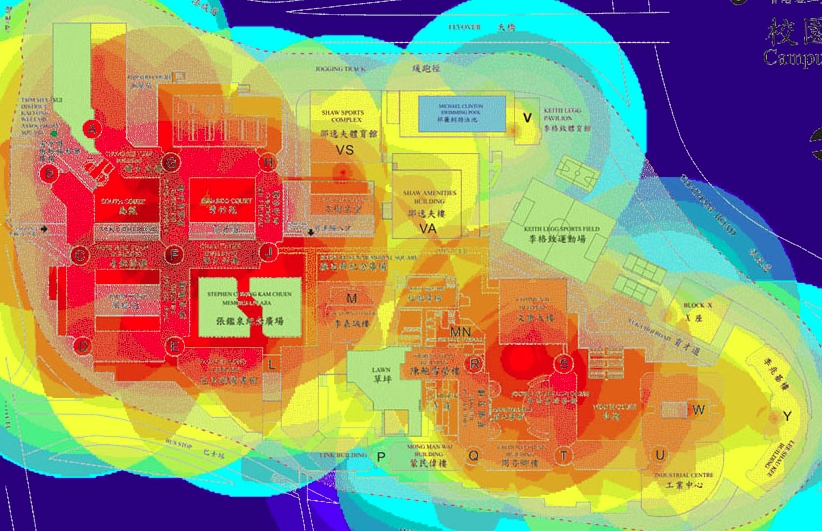
\includegraphics[width=.5\textwidth]{wifi-positioning}\end{figure}}
	\only<4>{\begin{figure}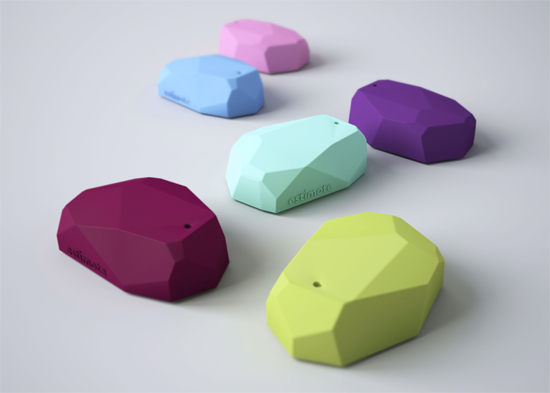
\includegraphics[width=.5\textwidth]{beacons}\end{figure}}
	\only<6>{
	  \begin{block}{RSSI --- received signal strenght indication}
	  	\begin{equation*}
	  		I \propto \frac{1}{r^2}
	  	\end{equation*}
	  \end{block}}
\end{frame}

\section{Mediacja}

\begin{frame}[fragile]
	\frametitle{Nowy pomysł --- mediacja}
	Zaangażowanie \alert{użytkownika} w proces mikro-lokalizacji.

	\only<2->{\begin{itemize}
		\only<2->{\item Zewnętrzny moduł lokalizacyjny (fizyczny).}
		\only<3->{\item Użytkownik pośrednio wybiera jedną z alternatyw\ldots}
		\only<4->{\item \ldots{} odpowiadając na pytania.}
	\end{itemize}}
\end{frame}

\begin{frame}[fragile]
	\frametitle{Generowanie pytań}
	\begin{itemize}
		\item Mapy GML/OpenGIS\only<2->{,}
		\only<2->{\item ontologia\only<3->{,}}
		\only<3->{\item wybranie cechy alternatyw o największym information gain\only<4->{,}}
		\only<4->{\item wygenerowanie konkretnego pytania z symbolicznej cechy\only<5->{.}}
	\end{itemize}
	\only<1>{\begin{figure}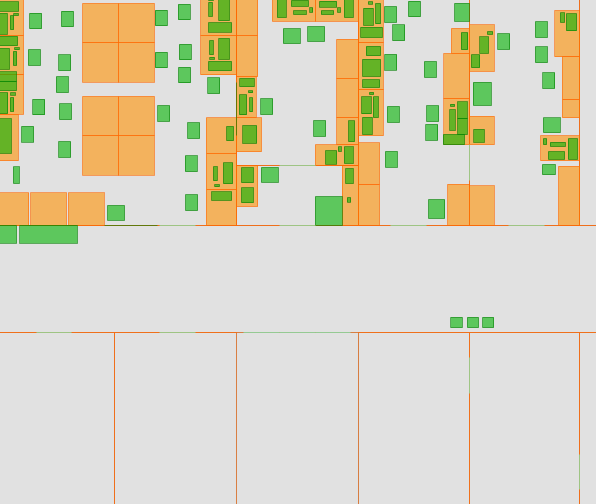
\includegraphics[width=.5\textwidth]{gml}\end{figure}}
	\only<2>{\begin{figure}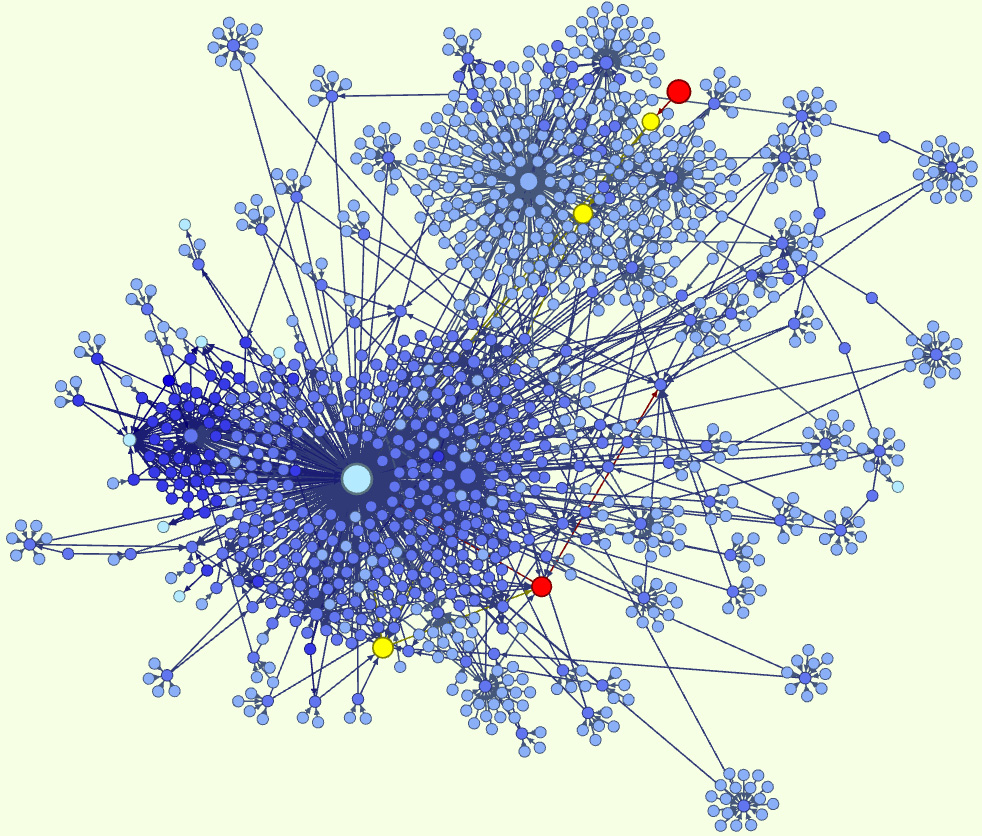
\includegraphics[width=.5\textwidth]{ontology}\end{figure}}
	\only<3>{\begin{equation*}
	    IG(T,a) = H(T) - H(T|a)
	  \end{equation*}}
	\only<4>{\begin{figure}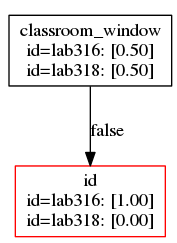
\includegraphics[width=.2\textwidth]{question-tree}\end{figure}}
	\only<5>{\begin{block}{Moduł regułowy}
	    Używany do wybierania cech (definiowania kosztów).
	  \end{block}}
\end{frame}

%\section{Conclusion}

\begin{frame}{Podsumowanie}
	\begin{itemize}
		\item Zwiększa dokładność (nawet do 100\%)\only<2->{,
		\item ale \alert{zły User Experience},
		\item miesce dla gamification, zabawy?}
		\only<3->{\item Najpewniej nie tędy droga\ldots
		\item \ldots{} a samą mediację można wykorzystać do czegoś innego.}
	\end{itemize}
\end{frame}

\plain{}

\end{document}
